\documentclass[12pt]{standalone}
\usepackage{tikz}
\usetikzlibrary{arrows.meta}
\usetikzlibrary{shapes.geometric}
\usetikzlibrary{shapes.symbols}
\usetikzlibrary{decorations,decorations.pathreplacing}
\usetikzlibrary{shadings}
\usetikzlibrary{backgrounds}
\usetikzlibrary{
  shapes,
  decorations.shapes,
  decorations.fractals,
  decorations.markings,
  shadows
}

\usepackage{setspace}
\usepackage{xcolor}

\definecolor{brightorange}{RGB}{255, 111, 0}

\begin{document}
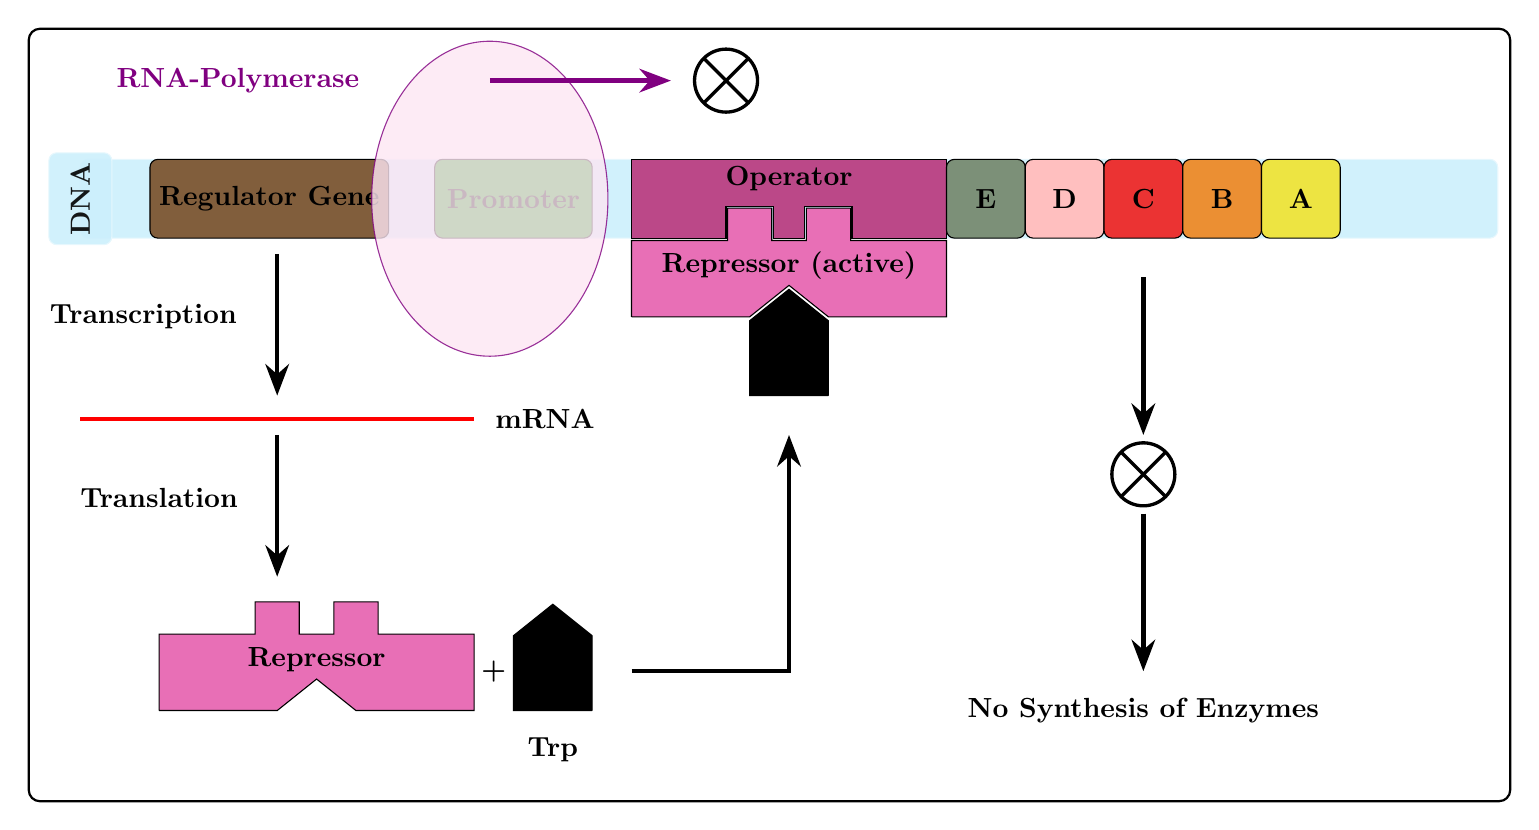
\begin{tikzpicture}[framed,background rectangle/.style={thick,draw=black, rounded corners},cross/.style={draw,path picture={
    \draw[black]
     (path picture bounding box.north west) -- (path picture bounding box.south east) 
     (path picture bounding box.south west) -- (path picture bounding box.north east);
    }}]
    %\draw[help lines] (-7,7) grid (7,-7); % Only for Development
  
    \node[shape=rectangle,
      rounded corners=1mm,
      draw=cyan!10,
      fill=cyan!20,
      fill opacity=0.9,
      minimum height = 1cm,
      minimum width = 18cm] at (0,0) {};
    \node[shape=rectangle,
      rounded corners=1mm,
      draw=cyan!10,
      fill=cyan!20,
      fill opacity=0.9,
      rotate=90,
      minimum height = 0.8cm,
      minimum width = 0.8cm] at (-9,0) {\textbf{DNA}};
    \node[shape=rectangle,
      rounded corners=1mm,
      draw=black,
      fill=brown!60!black!90,
      minimum height = 1cm,
      minimum width = 2cm] at (-6.6,0) {\textbf{Regulator Gene}};
    \node[shape=rectangle,
      rounded corners=1mm,
      draw=black,
      fill=green!60!black!90,
      minimum height = 1cm,
      minimum width = 2cm] at (-3.5,0) {\textbf{Promoter}};

    \node[shape=ellipse,
                      draw=violet,
                      rotate=90,
                      opacity=0.8,
                      fill=magenta!10,
                      minimum height = 3cm,
                      minimum width = 4cm] at (-3.8,0) {};
    \draw[-{Stealth[length=4mm]},ultra thick,draw=violet] (-3.8,1.5) -- (-1.5,1.5);
    \node [draw,circle,very thick,cross,minimum width=0.8cm] at (-0.8,1.5){}; 

    \node[shape=rectangle,
    text=violet,
    minimum height = 1cm,
    minimum width = 1cm] at (-7,1.5) {\textbf{RNA-Polymerase}};

    \draw[fill=magenta!70!black!90] 
      (-1,-0.5) -- (-2,-0.5) -- (-2,0.5) -- (2,0.5) -- 
      (2,-0.5) -- (0.8,-0.5) -- (0.8,-0.1) -- (0.2,-0.1) --
      (0.2,-0.5) -- (-0.2,-0.5) -- (-0.2,-0.1) -- (-0.8,-0.1) --
      (-0.8,-0.5) -- (-1,-0.5);

    \draw[fill=magenta!90!black!60]
      (-2,-1.5) -- (-2,-0.53) -- (-0.78,-0.53) -- (-0.78,-0.12) --
      (-0.22,-0.12) -- (-0.22,-0.53) -- (0.22,-0.53) -- (0.22,-0.12) --
      (0.782,-0.12) -- (0.782,-0.53) -- (2,-0.53) -- (2,-1.5) -- 
      (0.5,-1.5) -- (0,-1.1) -- (-0.5,-1.5) -- (-2,-1.5);

    \draw[fill=black]
      (0.5,-2.5) -- (-0.5,-2.5) -- (-0.5,-1.55) -- (0,-1.15) -- (0.5,-1.55) -- (0.5,-2.5);

    \node[shape=rectangle,
      minimum height = 1cm,
      minimum width = 1cm] at (0,-0.85) {\textbf{Repressor (active)}};

    \node[shape=rectangle,
      minimum height = 0.8cm,
      minimum width = 2cm] at (0,0.25) {\textbf{Operator}};

    \node[shape=rectangle,
      rounded corners=1mm,
      draw=black,
      fill=magenta!40!green!90,
      minimum height = 1cm,
      minimum width = 1cm] at (2.5,0) {\textbf{E}};
    \node[shape=rectangle,
      rounded corners=1mm,
      draw=black,
      fill=pink,
      minimum height = 1cm,
      minimum width = 1cm] at (3.5,0) {\textbf{D}};
    \node[shape=rectangle,
      rounded corners=1mm,
      draw=black,
      fill=red!90!black!80,
      minimum height = 1cm,
      minimum width = 1cm] at (4.5,0) {\textbf{C}};
    \node[shape=rectangle,
      rounded corners=1mm,
      draw=black,
      fill=orange!90!black!80,
      minimum height = 1cm,
      minimum width = 1cm] at (5.5,0) {\textbf{B}};
    \node[shape=rectangle,
      rounded corners=1mm,
      draw=black,
      fill=yellow!90!black!80,
      minimum height = 1cm,
      minimum width = 1cm] at (6.5,0) {\textbf{A}};

    \draw[-{Stealth[length=4mm]},ultra thick,draw=black] (4.5,-1) -- (4.5,-3);
    \node [draw,circle,very thick,cross,minimum width=0.8cm] at (4.5,-3.5){};
    \draw[-{Stealth[length=4mm]},ultra thick,draw=black] (4.5,-4) -- (4.5,-6);
    \node[shape=rectangle,
    minimum height = 1cm,
    minimum width = 1cm] at (4.5,-6.5) {\textbf{No Synthesis of Enzymes}};

    \draw[-{Stealth[length=4mm]},ultra thick,draw=black] (-6.5,-0.7) -- (-6.5,-2.5);
    \node[shape=rectangle,
      minimum height = 1cm,
      minimum width = 1cm] at (-8.2,-1.5) {\textbf{Transcription}};
      \draw[draw=red,ultra thick]
      (-9,-2.8) -- (-4,-2.8);
      \node[shape=rectangle,
      minimum height = 1cm,
      minimum width = 1cm] at (-3.1,-2.8) {\textbf{mRNA}};
    \draw[-{Stealth[length=4mm]},ultra thick,draw=black] (-6.5,-3) -- (-6.5,-4.8);
    \node[shape=rectangle,
      minimum height = 1cm,
      minimum width = 1cm] at (-8,-3.8) {\textbf{Translation}};
      
    \draw[fill=magenta!90!black!60]
      (-8,-6.5) -- (-8,-5.53) -- (-6.78,-5.53) -- (-6.78,-5.12) --
      (-6.22,-5.12) -- (-6.22,-5.53) -- (-5.78,-5.53) -- (-5.78,-5.12) --
      (-5.218,-5.12) -- (-5.218,-5.53) -- (-4,-5.53) -- (-4,-6.5) -- 
      (-5.5,-6.5) -- (-6,-6.1) -- (-6.5,-6.5) -- (-8,-6.5);
    \node[shape=rectangle,
      minimum height = 1cm,
      minimum width = 1cm] at (-6,-5.85) {\textbf{Repressor}};
    \draw[-{Stealth[length=4mm]},ultra thick,draw=black] (-2,-6) -- (0,-6) -- (0,-3);

  \node[shape=rectangle,
    minimum height = 1cm,
    minimum width = 1cm] at (-3.75,-6) {\textbf{+}};

  \node[shape=rectangle,
    minimum height = 1cm,
    minimum width = 1cm] at (-3,-7) {\textbf{Trp}};

    \draw[fill=black]
      (-2.5,-6.5) -- (-3.5,-6.5) -- (-3.5,-5.55) -- (-3,-5.15) -- (-2.5,-5.55) -- (-2.5,-6.5);

  \end{tikzpicture}
\end{document}